\documentclass{standalone}
\usepackage{tikz}
\begin{document}
    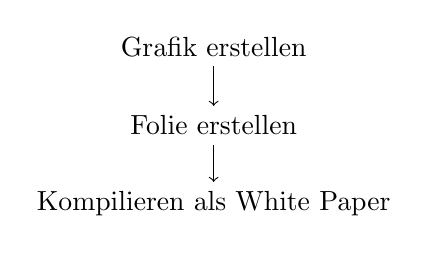
\begin{tikzpicture}
        \node (A) at (0,0) {Grafik erstellen};
        \node (B) at (0,-1) {Folie erstellen};
        \node (C) at (0,-2) {Kompilieren als White Paper};
        \draw[->] (A) -- (B);
        \draw[->] (B) -- (C);
    \end{tikzpicture}
\end{document}